\chapter{Evaluación experimental}
\label{capitulo3}
\lhead{Capítulo 3. \emph{Evaluación experimental}}

\section{Diseño experimental}

En este capítulo se describen todas las decisiones tomadas con respecto a la experimentación; esto incluye los parámetros usados para la entonación, las particiones hechas en la validación cruzada y la estratificación, el diseño de los experimentos donde se combinan las heurísticas con las metaheurísticas y finalmente se presentan los resultados de cada prueba realizada. 

Lo primero que se hace es entonar los algoritmos evolutivos para que devuelvan el mejor valor posible al probarse con los conjuntos de datos presentados en la sección 2.4. Para lograr la entonación, se usa \emph{irace}, presentado en la sección 2.6, con los parámetros de la tabla \ref{irace-param}. Se busca una configuración de parámetros para los problemas pequeños, medianos y grandes respectivamente.

\begin{table}[]
\centering
\begin{tabular}{l c}
\hline
Parámetros & irace \\
\hline
\hline
Iteraciones                                 &  1000, 400 y 100\\
Número decimales significativos             &    4            \\
Prueba estadística                          &  t-test         \\
Nivel de significancia para prueba estadística  &  0.05           \\
Frecuencia de la prueba estadística         &    1 iteración  \\
Número de configuraciones élites            &  automática     \\
Reinicialización por convergencia prematura &     Sí          \\
Modo elitista                               &     Sí          \\

\hline
\end{tabular}
\caption{Parámetros usados para \emph{irace}}
\label{irace-param}
\end{table}

Los parámetros a entonar son: número de iteraciones, cardinalidad de la población, probabilidad de cruce, probabilidad de mutación y tamaño del torneo. Los rangos válidos para cada parámetro se presentan en la tabla \ref{rangos}. La elección de los rangos se hace en base a los trabajos \cite{de2004reduccion,de2004reduccion,garcia2012prototype,garcia2008memetic,talbi2009metaheuristics}. Los resultados de la entonación se presentan en las tablas \ref{param-peq}, \ref{param-med} y \ref{param-grande}.

\begin{table}[]
\centering
\begin{tabular}{l c c}
\hline
Parámetros & Tipo de dato & Rangos \\
\hline
\hline

Población                & entero           &  [10,150]       \\
Probabilidad de cruce    & real             &  [0,1]          \\
Probabilidad de mutación & real             &  [0,0.01]      \\
Número del torneo        & entero           &  [1,10]         \\  

\hline
\end{tabular}
\caption{Rangos usados para los parámetros en la entonación}
\label{rangos}
\end{table}

\begin{table}[]
\centering
\begin{tabular}{l c c c c}
\hline
\multirow{2}{*}{\textsc{Parámetros}}
	& \multicolumn{4}{c}{\textsc{Algoritmos}} \\
	& GGA & SGA & MA & CHC \\
\hline
\hline
Iteraciones             &  1000    &  1000    &  1000      &  1000 \\
Población               &    70    &    90    &    21      &    33 \\
Prob. de Cruce          &   0.4837 &   0.9848 &     0.9496 &     - \\
Prob. de Mutación       &   0.0001 &  0.0057  &     0.0071 &     - \\
Número del torneo       &   -      &    3     &     1      &     - \\
\hline
\end{tabular}
\caption{Parámetros resultados de la entonación para los conjuntos pequeños}
\label{param-peq}
\end{table}


\begin{table}[]
\centering
\begin{tabular}{l c c c c}
\hline
\multirow{2}{*}{\textsc{Parámetros}}
	& \multicolumn{4}{c}{\textsc{Algoritmos}} \\
	& GGA & SGA & MA & CHC \\
\hline
\hline
Iteraciones             &  1000    &  1000    &  1000      &  1000 \\
Población               &    88    &    132   &    32      &    27 \\
Prob. de Cruce          &   0.5779 &   0.9859 &     0.9549 &     - \\
Prob. de Mutación       &   0.0001 &  0.0001  &     0.0004 &     - \\
Número del torneo       &   -      &    1     &     3      &     - \\
\hline
\end{tabular}
\caption{Parámetros resultados de la entonación para los conjuntos medianos}
\label{param-med}
\end{table}

\begin{table}[]
\centering
\begin{tabular}{l c c c c}
\hline
\multirow{2}{*}{\textsc{Parámetros}}
	& \multicolumn{4}{c}{\textsc{Algoritmos}} \\
	& GGA & SGA & MA & CHC \\
\hline
\hline
Iteraciones             &  1000    &  1000    &  1000      &  1000 \\
Población               &    102   &    122   &    35      &    37 \\
Prob. de Cruce          &   0.5158 &   0.9554 &     0.9698 &     - \\
Prob. de Mutación       &   0.0001 &  0.0078  &     0.0049 &     - \\
Número del torneo       &   -      &    7     &     3      &     - \\
\hline
\end{tabular}
\caption{Parámetros resultados de la entonación para los conjuntos grandes}
\label{param-grande}
\end{table}

Para la validación cruzada se usa k = 10 y se repite cada prueba 3 veces basándose en el trabajo de \emph{Cano, J.} en \cite{de2004reduccion}. Este esquema de validación cruzada se aplica a los conjuntos de tamaño pequeño como lo hacen en \cite{de2004reduccion}. Para la estratificación se adopta k = 10 para los conjuntos medianos y k = 50 para los conjuntos grandes, tal y como se determinan en \cite{cano2005stratification}, cuya idea es hacer que el algoritmo de PS no trabaje con más de 2000 instancias por estrato para reducir la cantidad a un conjunto de tamaño pequeño según la clasificación de la sección 2.5. Además, al igual que en la validación cruzada, las metaheurísticas utilizadas son estocásticas y por lo tanto, cada una de las k pruebas realizadas se repite 3 veces, con lo que se regresa el promedio de todas las pruebas realizadas como resultado.

Una vez obtenido los distintos parámetros para cada metaheurística, se procede con el experimento principal, el cual consiste en mejorar la población inicial de las metaheurísticas GGA, SSGA, MA y CHC por medio de las heurísticas CNN, ENN, RSS y sus combinaciones.

Para presentar los resultados, se usan tablas que contienen los promedios en \emph{accuracy}, \emph{kappa}, reducción, \emph{accuracy} + reducción y tiempo de cómputo medido en segundos para cada heurística. \emph{Accuracy y kappa} se miden sobre los conjuntos de entrenamiento y validación, la reducción mide el porcentaje de instancias eliminadas del conjunto original; a mayor \emph{accuracy, kappa} y reducción mejor es el algoritmo. Las pruebas fueron realizadas para los conjuntos pequeños, medianos y grandes por separado. Además, para determinar si una metaheurística es mejor que otra se utiliza una prueba de \emph{Wilcoxon} de rango con signo con un nivel de significacia de 1\%, donde la hipótesis nula implica que las medidas son estadísticamente iguales y la hipótesis alternativa indica que existe una diferencia real entre las medidas. 


Se selecciona la mejor metahuerística en base a \emph{accuracy} + reducción, donde el \emph{accuracy} que se toma en cuenta es el del conjunto de validación (\emph{test}); si hay metaheurísticas estadísticamente similares, se selecciona aquella que utilice menos tiempo para dar un resultado. Además, se descartan aquellas metaheurísticas que tienen un \emph{kappa} en el conjunto de validación por debajo del 50\% porque esto indica que el clasificador etiqueta en mayor medida de manera aleatoria y no gracias a la información inherente a los datos. La mejor metaheurística se encuentra en negrita en cada tabla.

Los experimentos fueron hechos con un procesador Intel(R) Core(TM) i5-3470 CPU @ 3.20GHz, 4 procesadores y 4GB de memoria RAM. Se utilizó C++ como lenguaje de programación y se compiló con GCC v.7.3.0.

\section{Resultados}

\subsection{Heurísticas}

En esta sección se busca estudiar el comportamiento de CNN, ENN y RSS al ser usados para resolver el problema de selección de prototipos sobre conjuntos de datos de tamaño pequeño, mediano y grande. De los resultados obtenidos, se espera determinar cuál heurística presenta el mayor nivel de \emph{accuracy} + reducción; además se busca evaluar el tiempo de cómputo de cada heurística.


\begin{table}[h!]
\centering
\begin{adjustbox}{max width =\textwidth}
\begin{tabular}{l c c c c c c c}
\hline
\multirow{2}{*}{\textsc{Algoritmo}}
	& \multicolumn{2}{c}{\textsc{Accuracy}}
	& \multicolumn{2}{c}{\textsc{Kappa}}
	& \textsc{Reducción}
	& \textsc{Acc + Red}
	& \textsc{Tiempo (seg)} \\
	& Training & Test
	& Training & Test \\ 
\hline
\hline

Pequeños\\
\textbf{CNN} & \textbf{90.93} & \textbf{74.47} & \textbf{83.96} & \textbf{54.04} & \textbf{73.80} & \textbf{148.27} & \textbf{0.1351} \\
ENN & 85.63 & 79.24 & 73.19 & 61.20 & 25.91 & 105.15 & 0.1815 \\
RSS & 83.63 & 74.99 & 69.97 & 54.26 & 73.08 & 148.07 & 0.1231 \\

\hline

Medianos\\
\textbf{CNN} & \textbf{89.44} & \textbf{78.23} & \textbf{76.11} & \textbf{56.13} & \textbf{74.37} & \textbf{152.6} & \textbf{0.7108} \\
ENN & 84.02 & 79.99 & 68.42 & 58.63 & 28.61 & 108.6 & 1.2668 \\
RSS & 86.19 & 79.22 & 68.22 & 55.24 & 64.77 & 143.99 & 0.9201 \\

\hline

Grandes\\
\textbf{CNN} & \textbf{88.18} & \textbf{81.58} & \textbf{73.96} & \textbf{55.87} & \textbf{81.83} & \textbf{163.41} & \textbf{3.2853} \\
ENN & 93.55 & 88.95 & 79.38 & 64.63 & 14.95 & 103.9 & 6.1658 \\
RSS & 91.76 & 87.31 & 74.11 & 60.07 & 72.36 & 159.67 & 10.7264 \\


\hline
\end{tabular}
\end{adjustbox}
\caption{Promedios de los resultados obtenidos en las distintas métricas para cada heurística}
\label{heu}
\end{table}

Al estudiar los resultados presentes en la tabla \ref{heu}, se puede destacar que CNN es la heurística que tiene los mayores niveles de \emph{accuracy} + reducción. Esto sucede porque CNN elige sólo las instancias limítrofes entre clases para construir el conjunto $S$, eliminando la mayoría de las instancias que se concentran en la parte interna del espacio.

Al evaluar los tiempos de cómputo presentes en la tabla \ref{heu} se pueden observar los siguientes detalles:

\begin{itemize}

\item CNN es la heurística más rápida y es la que mejor escala a conjuntos de tamaño grande. Su rapidez sucede porque el algoritmo empieza con un conjunto vacío y agrega instancias conforme a los errores de clasificación que encuentra en cada iteración, deteniéndose cuando logra pasar una iteración sin errores, este esquema le permite a CNN terminar rápidamente en la mayoría de los casos, independientemente del tamaño del conjunto a reducir. Se debe acotar que CNN, siendo un algoritmo con componentes estocásticos, puede tardar más del tiempo esperado en dar una solución, porque, dependiendo del orden de presentación de las instancias, CNN puede llegar a necesitar varios iteraciones sobre el conjunto original para terminar; para casos patológicos, CNN puede llegar a tener una complejidad de $O(n^2*log(n))$, cuando el tiempo esperado normalmente es de $O(n*log(n))$.

\item ENN presenta los tiempos más largos en dar una respuesta para los conjuntos pequeños y medianos. El tiempo adicional que le toma a ENN devolver una solución en comparación a CNN se debe a que ENN empieza con el conjunto original en su totalidad y en cada iteración elimina una instancia que no concuerda con la clase de su vecino más cercano. Sin embargo, como ENN sólo tiene que revisar cada instancia una sola vez, puede terminar en un buen tiempo inclusive con los conjuntos grandes. ENN tiene una complejidad de $O(n*log(n))$  

\item RSS es la heurística que presenta el crecimiento en tiempo de cómputo más pronunciado, ya que se requiere para terminar con un conjunto grande 10 veces más el tiempo requerido por un conjunto mediano. Este detalle de escalabilidad se debe a que RSS primero debe ordenar todas las instancias según la distancia a sus enemigos más cercanos, lo cual domina el tiempo del algoritmo y asintóticamente lo vuelve $O(n*log(n))$. 

\end{itemize}

Una vez considerado los tiempos, se concluye que CNN es la mejor heurística para resolver el problema de selección de prototipos para los conjuntos de los tres tamaños. Esto gracias a que presenta los mayores niveles de \emph{accuracy} + reducción y utiliza la menor cantidad de tiempo para dar una respuesta. 


\subsection{Metaheurísticas}

En esta sección se estudia el comportamiento de GGA, SSGA, MA y CHC, con población inicial aleatoria, al resolver el problema de selección de instancias sobre conjuntos pequeños, medianos y grandes. El objetivo es determinar cuál algoritmo presenta el mayor nivel de \emph{accuracy} + reducción para los conjuntos de los distintos tamaños. Además, se estudia el tiempo que requiere cada algoritmo en dar una solución.


\begin{table}[h!]
\centering
\begin{adjustbox}{max width =\textwidth}
\begin{tabular}{l c c c c c c c}
\hline
\multirow{2}{*}{\textsc{Algoritmo}}
	& \multicolumn{2}{c}{\textsc{Accuracy}}
	& \multicolumn{2}{c}{\textsc{Kappa}}
	& \textsc{Reducción}
	& \textsc{Acc + Red}
	& \textsc{Tiempo (seg)} \\
	& Training & Test
	& Training & Test \\ 
\hline
\hline

Pequeños\\
GGA  & 83.12 & 75.25 & 70.17 & 55.57 & 55.32 & 130.57 & 12.8250 \\
SSGA & 86.54 & 77.16 & 76.35 & 59.17 & 84.32 & 161.48 & 0.6655 \\
MA   & 85.70 & 79.18 & 74.40 & 62.16 & 95.61 & 174.79 & 4.1047 \\
\textbf{CHC}  & \textbf{84.46} & \textbf{78.43} & \textbf{71.72} & \textbf{60.84} & \textbf{94.66} & \textbf{173.09} & \textbf{0.5266} \\

\hline

Medianos\\
GGA  & 87.02 & 79.82 & 73.75 & 58.12 & 56.41 & 136.23 & 110.0812 \\
SSGA & 84.31 & 80.29 & 66.76 & 58.71 & 83.92 & 164.21 & 3.5589 \\
MA   & 80.57 & 79.08 & 58.25 & 55.64 & 96.24 & 175.32 & 73.3461 \\
\textbf{CHC}  & \textbf{83.13} & \textbf{81.15} & \textbf{63.47} & \textbf{59.86} & \textbf{94.55} & \textbf{175.7}  & \textbf{2.8843} \\

\hline
Grandes\\
GGA  & 93.16 & 86.44 & 79.94 & 60.14 & 50.50 & 136.94 & 672.0273 \\
SSGA & 89.11 & 87.43 & 69.53 & 62.01 & 80.56 & 167.99 & 27.6637 \\
MA   & 89.04 & 89.99 & 64.99 & 65.10 & 99.73 & 189.72 & 256.1432 \\
\textbf{CHC}  & \textbf{89.61} & \textbf{89.34} & \textbf{66.14} & \textbf{65.06} & \textbf{96.15} & \textbf{185.76} & \textbf{16.8665} \\

\hline
\end{tabular}
\end{adjustbox}
\caption{Promedios de los resultados obtenidos en las distintos métricas para cada metaheurística}
\label{meta}

\end{table}

Al estudiar los resultados obtenidos en la tabla \ref{meta}, se puede destacar los siguientes puntos:

CHC y MA presentan los mayores niveles de \emph{accuracy} + reducción, para los conjuntos pequeños, medianos y grandes. Esto se atribuye a las herramientas que tiene cada algoritmo para hacer la mejor selección de instancias posible. MA tiene su función de optimización que elimina todas las instancias posibles sin perjudicar el \emph{accuracy}, lo que permite mejorar al máximo cada cromosoma de la población; mientras que CHC tiene su mecanismo de prevención de incesto que crea cromosomas lo más distinto posible de los padres, además de tener la capacidad de reiniciar su población, tomando como base el mejor cromosoma encontrado, para evitar la convergencia prematura de la misma.

SSGA y GGA presentan niveles similares de \emph{accuracy y kappa} que MA y CHC. Sin embargo, presentan tasas de reducción menores a estos últimos porque tienen una selección de instancias menos informadas. Además, cabe destacar los siguientes puntos:

\begin{itemize}

\item GGA presenta los niveles más bajos de reducción, esto ocurre porque no posee mecanismos de preservación elitistas como en el caso de CHC. GGA se caracteriza por perder toda la información acumulada en una generación de cromosomas (excepto el mejor), eliminando cromosomas que podrían generar mejores soluciones si se les diera más oportunidades de ser cruzados. Además, GGA carece de procesos de intensificación como los tiene MA, lo cual vuelve más difícil la eliminación de instancias.

\item SSGA presenta mejores niveles de reducción a los obtenidos por GGA porque usa un método simple de elitismo, en el cual en cada iteración sólo se generan dos cromosomas nuevos (a diferencia de una población entera) y éstos sólo suplantan a sus padres si son mejores. Este mecanismo permite que la cantidad de instancias disminuya paulatinamente hasta llegar a la convergencia de la población.

\end{itemize}


En relación a los tiempos de cómputo se puede destacar:

\begin{itemize}

\item CHC es la metaheurística que necesita menos tiempo en dar una solución. Esto se debe a su operador de cruce, el cual tarda tiempo lineal ($O(n)$) y permite hacer una búsqueda diversificada del espacio de soluciones de manera inteligente, ya que, a partir de unos cromosomas seleccionados de manera elitista, genera nuevos cromosomas que son lo más distinto posible, mientras mantiene algunas cualidades (las cuales se esperan que sean buenas) de sus padres. Estos detalles hacen posible la obtención de buenos resultados rápidamente.

\item SSGA es otra metaheurística que no necesita mucho tiempo en dar una solución. La razón de esto es parecida a la de CHC, ya que el operador de cruce toma tiempo lineal y en cada iteración sólo se generan 2 cromosomas, lo cual lleva al algoritmo a terminar rápidamente.

\item MA tarda significativamente más en regresar una solución en comparación a CHC y SSGA. Para los conjuntos pequeños, MA tarda 7 veces más que CHC; para los conjuntos medianos, MA tarda 25 veces más que CHC y para los conjuntos grandes, MA tarda 15 veces más. Esta diferencia en tiempo se debe al proceso de optimización interna que usa MA en cada iteración, el cual es $O(n^2)$.

\item GGA es la metaheurística que más tarda en dar una solución. Esto se debe a que en cada iteración, GGA debe generar una población de cromosomas nuevo, a diferencia de SSGA que sólo genera dos cromosomas.

\item CHC y SSGA son las metaheurísticas que mejor escalan a los conjuntos grandes, ya que mantienen los tiempos de ejecución por debajo de 30 segundos, teniendo valores no muy alejados de los tiempos obtenidos por las heurísticas. Por otra parte, GGA y MA sobrepasan los 200 segundos en tiempo de cómputo, lo cual es 20 veces más lo que tardan CNN, ENN y RSS. Sin embargo, hay que tomar en cuenta que la estratificación ayuda a reducir significativamente los tiempos de cómputo de las cuatro metaheurísticas, al punto de que es factible aplicar los cuatro algoritmos a los conjuntos grandes; ya que en trabajos como los realizados por \emph{Cano, J. et al.} en \cite{garcia2008memetic} y \cite{garcia2012prototype} no se pudo probar estos algoritmos sin el uso de estratificación por la gran cantidad de tiempo que tomarían en devolver una respuesta.

\end{itemize}


\begin{figure}[h!]

	\centering
	\subfigure[\emph{Accuracy} + reducción]{\label{fig:a}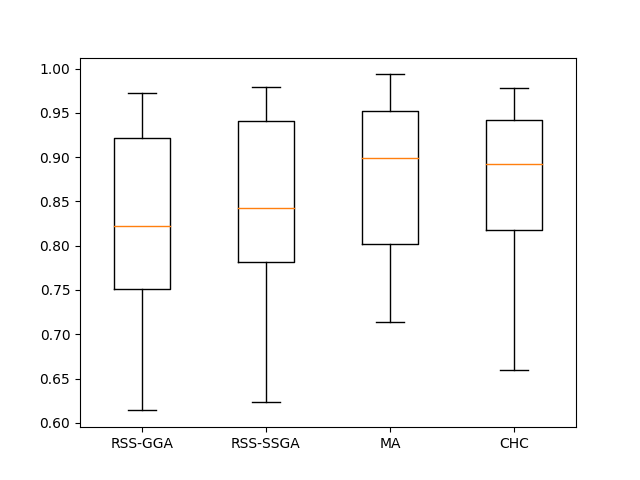
\includegraphics[scale=0.45]{acc_small.png}}
	\subfigure[\emph{kappa} + reducción]{\label{fig:b}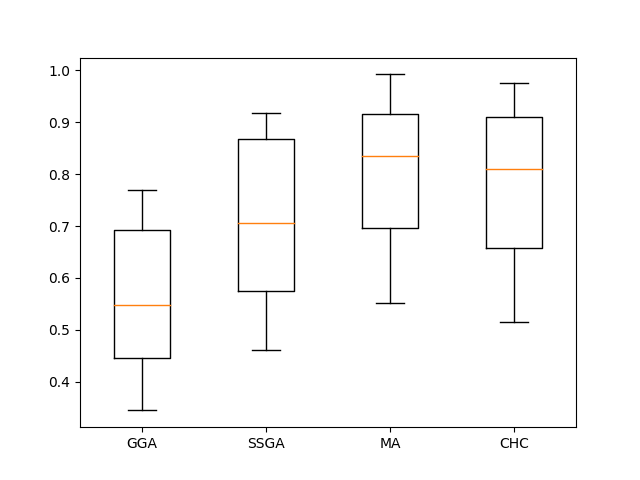
\includegraphics[scale=0.45]{kappa_small.png}}

\caption{Boxplots de las metaheurísticas para los conjuntos pequeños}
\label{small-heuristics}
\end{figure}

\begin{figure}[h!]

	\centering
	\subfigure[\emph{Accuracy} + reducción]{\label{fig:a}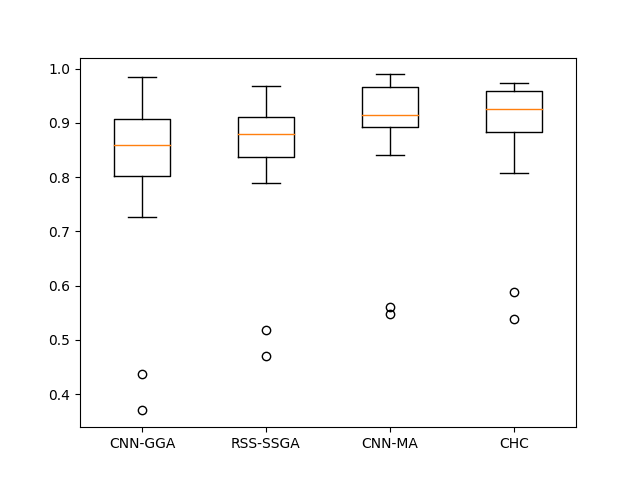
\includegraphics[scale=0.45]{acc_medium.png}}
	\subfigure[\emph{kappa} + reducción]{\label{fig:b}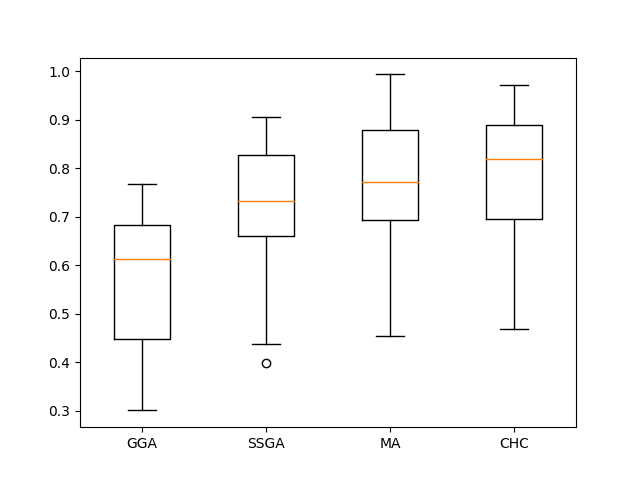
\includegraphics[scale=0.45]{kappa_medium.png}}

\caption{Boxplots de las metaheurísticas para los conjuntos medianos}
\label{medium-heuristics}
\end{figure}

Las figuras \ref{small-heuristics} y \ref{medium-heuristics} muestran que cuando se toma en cuenta la combinación lineal de \emph{accuracy} + reducción y \emph{kappa} + reducción, MA y CHC presentan los niveles más elevados. Cabe destacar que las tablas \ref{wilcox-meta-peq} y \ref{wilcox-meta-med} del Apéndice A muestran que los p-valores de la comparación entre MA y CHC para los conjuntos pequeños son 6.934e-02 para \emph{accuracy} + reducción y  7.80e-02 para \emph{kappa} + reducción. Por su parte, para los conjuntos medianos se tiene 6.009e-01 y 7.172e-01 respectivamente; lo cual implica que MA y CHC son estadísticamente similares. 

De acuerdo a la información presentada anteriormente, se puede concluir que CHC es la mejor metaheurística para resolver el problema de selección de prototipos para los conjuntos pequeños, medianos y grandes. Ya que, junto a MA presenta los valores más elevados de \emph{accuracy, kappa} y reducción, con la peculiaridad de que es la metaheurística que menos tiempo tarda en culminar. Lo cual lo hace el candidato ideal al momento de aumentar el tamaño de los conjuntos de datos.  

\subsection{Combinaciones de las metaheurísticas}

Después del proceso anterior, el paso a seguir es la combinación de las heurísticas con las metaheurísticas. La idea es evaluar las combinaciones de cada metaheurística por separado, de tal manera de que se se identifique cuál heurística beneficia más a la metaheurística. La notación en la columna de ``\textsc{Algoritmo}'' indica primero qué heurística se usó para inicializar la población y le sigue la metaheurística usada; un ejemplo es CNN-GGA, que indica que CNN es la heurística usada para inicializar la población de la metaheurística GGA. Para el caso de usar una población incial aleatoria, se coloca simplemente el nombre de la metaheurística.


\subsubsection{Conjuntos pequeños}

En esta sección se estudia el comportamiento de las combinaciones de GGA, SSGA, MA y CHC al resolver el problema de selección de instancias sobre conjuntos pequeños. El objetivo es determinar cuál algoritmo presenta el mayor nivel de \emph{accuracy} + reducción. Además, se estudia el tiempo que requiere cada algoritmo en dar una solución.


\begin{table}[h!]
\centering
\begin{adjustbox}{max width =\textwidth}
\begin{tabular}{l c c c c c c c}
\hline
\multirow{2}{*}{\textsc{Algoritmo}}
	& \multicolumn{2}{c}{\textsc{Accuracy}}
	& \multicolumn{2}{c}{\textsc{Kappa}}
	& \textsc{Reducción}
	& \textsc{Acc + Red}
	& \textsc{Tiempo (seg)} \\
	& Training & Test
	& Training & Test \\ 
\hline
\hline

CNN-GGA     & 57.36 & 49.11 & 35.25 & 21.51 & 74.91 & 124.02 & 33.4671 \\
\textbf{ENN-GGA}     & \textbf{85.33} & \textbf{78.91} & \textbf{73.27} & \textbf{60.93} & \textbf{26.11} & \textbf{105.02} & \textbf{14.6024} \\
RSS-GGA     & 66.26 & 61.77 & 40.44 & 32.63 & 77.17 & 138.94 & 21.5376 \\
CNN-RSS-GGA & 78.83 & 68.09 & 63.53 & 44.72 & 62.21 & 130.3 & 43.1002 \\
ENN-RSS-GGA & 89.73 & 78.72 & 81.82 & 60.63 & 19.94 & 98.66 & 36.5439 \\

\hline

CNN-SSGA & 87.91 & 76.95 & 78.40 & 58.15 & 84.25 & 161.2 & 1.2187 \\
ENN-SSGA & 87.33 & 79.19 & 76.83 & 61.12 & 78.23 & 157.42 & 0.8601 \\
\textbf{RSS-SSGA} & \textbf{85.81} & \textbf{77.26} & \textbf{74.60} & \textbf{59.05} & \textbf{89.58} & \textbf{166.84} &\textbf{1.0116} \\
CNN-RSS-SSGA & 88.08 & 77.42 & 78.84 & 59.74 & 83.73 & 161.15 & 1.9109 \\
EEN-RSS-SSGA & 88.43 & 78.90 & 79.04 & 61.34 & 75.86 & 154.76 & 1.6563 \\

\hline

CNN-MA & 86.53 & 79.87 & 75.19 & 63.07 & 94.86 & 174.73 & 5.9638 \\
\textbf{ENN-MA} & \textbf{86.66} & \textbf{79.30} & \textbf{75.76} & \textbf{62.15} & \textbf{95.34} & \textbf{174.64} & \textbf{4.2491} \\
RSS-MA & 84.46 & 77.95 & 71.37 & 59.03 & 96.30 & 174.25 & 4.6391 \\
CNN-RSS-MA  & 86.39 & 78.48 & 75.38 & 60.90 & 95.07 & 173.55 & 8.9884 \\
ENN-RSS-MA & 87.36 & 79.42 & 77.16 & 62.68 & 94.74 & 174.16 & 8.3942 \\

\hline

CNN-CHC & 84.95 & 78.12 & 72.69 & 60.27 & 93.85 & 171.97 & 0.7891 \\
ENN-CHC & 84.29 & 78.63 & 71.79 & 61.32 & 94.24 & 172.87 & 0.7445 \\
\textbf{RSS-CHC} & \textbf{83.83} & \textbf{77.79} & \textbf{69.63} & \textbf{58.36} & \textbf{95.46} & \textbf{173.25} & \textbf{0.7137} \\
CNN-RSS-CHC  & 84.42 & 77.94 & 70.99 & 58.64 & 94.37 & 172.31 & 1.1144 \\
ENN-RSS-CHC & 84.84 & 78.46 & 72.24 & 60.30 & 93.33 & 171.79 & 1.0723 \\

\hline
\end{tabular}
\end{adjustbox}
\caption{Promedios de los resultados obtenidos en las distintas métricas para las distintas combinaciones de cada metaheurística sobre los conjuntos pequeños}
\label{peq-all}

\end{table}

Al estudiar los resultados obtenidos en la tabla \ref{peq-all}, se pueden destacar los siguientes aspectos observados de las combinaciones de GGA:

\begin{itemize}

\item CNN-GGA y RSS-GGA presentan los niveles más bajos de \emph{kappa}, lo cual significa que los dos algoritmos generan conjuntos que incluyen principalmente elementos de la clase mayoritaria, dejando pocos representantes de las clases minoritarias que no ayudan a la correcta clasificación de las mismas. Estos valores por debajo del 35\% implican que entre los conjuntos pequeños hay conjuntos que están sesgados hacia una o más clases y los conjuntos construidos por CNN-GGA y RSS-GGA no logran representar correctamente las clases minoritarias.

\item CNN-GGA, RSS-GGA y CNN-RSS-GGA no se toman en cuenta para definir la mejor combinación de GGA por presentar un \emph{kappa} inferior al 50\%.

\item{ENN-GGA} presenta los mayores niveles de \emph{accuracy} + reducción. Esto se debe a que es la combinación que preserva la mayor cantidad de instancias y por lo tanto el resultado mantiene un buen nivel de representación del conjunto original. Sin embargo GGA carece de los medios para realizar una reducción significativa de un conjunto densamente poblado, lo cual afecta la tasa de reducción.

\item ENN-GGA y RSS-GGA son las combinaciones que menos tiempo toman en dar un resultado porque, tanto ENN como RSS, tienen una complejidad de $O(n*log(n))$ los cuales les permite devolver una respuesta rápidamente.

\item CNN-GGA tarda más que ENN-GGA y que RSS-GGA por una combinación de factores que incluyen: los componentes estocásticos de CNN, que pueden ocasionar una elevada cantidad de iteraciones hasta converger a un conjunto; y la probabilidad de cruce elegida para GGA, la cual es de 48.37\%, lo que trae como consecuencia que pasen muchas iteraciones intentando cruzar cromosomas para formar todos los elementos de cada generación. Cabe destacar que el promedio de tiempo de cómputo de CNN-GGA se ve afectado por dos casos atípicos: \emph{Banknote} y \emph{Winsconsin} para los cuales se reportan 280.39 segundos y 272.64 segundos (véase tabla \ref{res-peq-cnn-gga} en el apéndice B) para que el algoritmo culmine.

\end{itemize}

De las observaciones anteriores se puede concluir que ENN-GGA es la mejor combinación de GGA, ya que obtiene los mayores niveles de \emph{accuracy y kappa} en el menor tiempo. Cabe acotar que aunque RSS-GGA, CNN-GGA y CNN-RSS-GGA tienen un mayor nivel de \emph{accuracy + reducción}, obtienen un nivel de \emph{kappa} inferior al 50\%, lo que indica que el clasificador no tiene información útil para etiquetar las instancias correctamente y toma la mayoría de sus decisiones al azar.

Al pasar a los resultados obtenidos por las combinaciones de SSGA, se puede observar que RSS-SSGA presenta los mayores niveles de \emph{accuracy} + reducción, gracias a la selección de instancias realizada por RSS, la cual introduce variedad en la búsqueda de SSGA. Además, los tiempos más cortos son los obtenidos por ENN-SSGA y RSS-SSGA. 

De las consideraciones anteriores, se puede concluir que RSS-SSGA es la mejor combinación de SSGA, ya que presenta el mayor nivel de \emph{accuracy} + reducción y se encuentra entre las combinaciones más rápidas. Cabe acotar que cuando se compara con CNN-SSGA (la combinación con valores más cercanos RSS-SSGA) usando la prueba \emph{Wilcoxon}, se obtiene un p-valor de 1.186e-03 (ver tabla \ref{wilcox-SSGA-peq} en el apéndice A), lo que implica que existe una diferencia real en los promedios y por lo tanto la diferencia de 5.33\% en la tasa de reducción es significativa.

Al evaluar los resultados obtenidos por las combinaciones de MA y CHC, se observa que todas presentan \emph{accuracy + reducción} similares. Los p-valores de las tablas \ref{wilcox-MA-peq} y \ref{wilcox-CHC-peq} en el apéndice A corroboran este hecho. Por lo tanto, se concluye que MA y CHC son metaheurísticas capaces de obtener resultados consistentes independientemente de la población inicial que utilicen. Razón por la cual las mejores combinaciones se eligen en base al tiempo de cómputo, que en este caso las que tardan menos tiempo son ENN-MA y RSS-CHC.

En la tabla \ref{peq-best-all} se comparan las mejores combinaciones de cada metaheurística con su versión original (población inicial aleatoria). La idea es determinar si la mejor combinación representa una mejoría sobre la versión original. De esta tabla se puede llegar a las siguientes conclusiones:

\begin{table}[h!]
\centering
\begin{adjustbox}{max width =\textwidth}
\begin{tabular}{l c c c c c c c}
\hline
\multirow{2}{*}{\textsc{Algoritmo}}
	& \multicolumn{2}{c}{\textsc{Accuracy}}
	& \multicolumn{2}{c}{\textsc{Kappa}}
	& \textsc{Reducción}
	& \textsc{Acc + Red}
	& \textsc{Tiempo (seg)} \\
	& Training & Test
	& Training & Test \\ 
\hline
\hline

\textbf{GGA}  & \textbf{83.12} & \textbf{75.25} & \textbf{70.17} & \textbf{55.57} & \textbf{55.32} & \textbf{130.57} & \textbf{12.8250} \\
ENN-GGA     & 85.33 & 78.91 & 73.27 & 60.93 & 26.11 & 105.02 & 14.6024 \\

\hline

SSGA & 86.54 & 77.16 & 76.35 & 59.17 & 84.32 & 161.48 & 0.6655 \\
\textbf{RSS-SSGA} & \textbf{85.81} & \textbf{77.26} & \textbf{74.60} & \textbf{59.05} & \textbf{89.58} & \textbf{166.84} &\textbf{1.0116} \\


\hline

\textbf{MA}   & \textbf{85.70} & \textbf{79.18} & \textbf{74.40} & \textbf{62.16} & \textbf{95.61} & \textbf{174.79} & \textbf{4.1047} \\
ENN-MA & 86.66 & 79.30 & 75.76 & 62.15 & 95.34 & 174.64 & 4.2491 \\


\hline

\textbf{CHC}  & \textbf{84.46} & \textbf{78.43} & \textbf{71.72} & \textbf{60.84} & \textbf{94.66} & \textbf{173.09} & \textbf{0.5266} \\
RSS-CHC & 83.83 & 77.79 & 69.63 & 58.36 & 95.46 & 173.25 & 0.7137 \\


\hline
\end{tabular}
\end{adjustbox}
\caption{Comparación entre los resultados de las métricas obtenidas por la metahuerística original y la mejor combinación para los conjuntos pequeños}
\label{peq-best-all}

\end{table}

\begin{itemize}
 
\item ENN-GGA presenta un menor valor de \emph{accuracy} + reducción que GGA, debido a que posee una tasa menor de reducción. Por lo tanto, ENN-GGA representa una desmejora con respecto a GGA.

\item RSS-SSGA presenta un mayor valor de \emph{accuracy} + reducción que SSGA, principalmente por tener una tasa de reducción 5.26\% por encima de SSGA, mientras mantiene niveles similares de \emph{accuracy y kappa}. Al hacer la prueba de \emph{Wilcoxon} para \emph{accuracy} + reducción se obtiene el p-valor 1.941e-04 (ver tabla \ref{wilcox-SSGA-peq} en el apéndice A), lo que significa que hay una diferencia real entre RSS-SSGA y SSGA. Estas razones justifican el tiempo adicional de cómputo de RSS-GGA, por lo que se determina como una mejoría real sobre SSGA.

\item Los valores de \emph{accuracy} + reducción son similares entre MA y ENN-MA. El p-valor de la prueba estadística es 5.629e-01 (ver tabla \ref{wilcox-MA-peq} en el apéndice A), por lo que no hay una diferencia significativa. Por lo tanto, ENN-MA no representa una mejora sobre MA y sólo aumenta el tiempo de cómputo.

\item  Los valores de \emph{accuracy} + reducción son similares entre CHC y RSS-CHC. El p-valor de la prueba estadística es 7.982e-01 (ver tabla \ref{wilcox-CHC-peq} en el apéndice A), por lo que no hay una diferencia significativa. Por lo tanto, RSS-CHC no representa una mejora sobre CHC y sólo aumenta el tiempo de cómputo.

\end{itemize}

\newpage

En la tabla \ref{rank-peq} se ordenan las metaheurísticas por el rango en el que se encuentran al compararse entre ellas por \emph{accuracy} + reducción y \emph{kappa} + reducción. Mientras menor sea el rango, más elevados son las métricas. En la columna de ``Mejor'' se contabiliza los conjuntos para los cuales dicha metaheurística obtuvo los mejores resultados.

\begin{table}[h!]
\centering
\begin{adjustbox}{max width =\textwidth}
\begin{tabular}{l c c|l c c}
\hline
\multicolumn{3}{c|}{\textsc{Accuracy + Reducción}}
	& \multicolumn{3}{c}{\textsc{Kappa + Reducción}} \\
\hline
Algoritmo & Rango & Mejor & Algoritmo & Rango & Mejor \\
\hline
\hline

MA           & 5.38  & 5 & CNN-MA       & 5.26  & 4  \\
ENN-MA       & 5.46  & 2 & ENN-MA       & 5.53  & 0 \\
CNN-MA       & 5.57  & 4 & MA           & 5.57  & 5 \\
RSS-MA       & 6.07  & 6 & ENN-RSS-MA   & 6.00  & 3 \\
ENN-RSS-MA   & 6.30  & 3 & RSS-MA       & 6.76  & 6 \\
RSS-CHC      & 6.80  & 1 & CNN-RSS-MA   & 7.07  & 0 \\
CNN-RSS-MA   & 6.96  & 0 & ENN-CHC      & 7.46  & 2 \\
CHC          & 7.07  & 0 & CHC          & 7.50  & 1 \\
ENN-CHC      & 7.53  & 0 & RSS-CHC      & 7.96  & 1 \\
CNN-RSS-CHC  & 7.65  & 2 & CNN-RSS-CHC  & 8.07  & 2 \\
ENN-RSS-CHC  & 7.88  & 2 & ENN-RSS-CHC  & 8.26  & 1  \\
CNN-CHC      & 8.73  & 1 & CNN-CHC      & 8.84  & 1  \\
RSS-SSGA     & 12.07 & 0 & RSS-SSGA     & 11.92 & 0  \\
CNN-SSGA     & 14.53 & 0 & SSGA         & 14.30 & 0  \\
SSGA         & 14.88 & 0 & CNN-RSS-SSGA & 14.26 & 0  \\
CNN-RSS-SSGA & 15.07 & 0 & CNN-SSGA     & 14.46 & 0  \\
ENN-SSGA     & 16.11 & 0 & ENN-SSGA     & 15.26 & 0  \\
ENN-RSS-SSGA & 17.26 & 0 & ENN-RSS-SSGA & 16.42 & 0  \\
RSS-GGA      & 19.11 & 0 & GGA          & 20.15 & 0  \\
GGA          & 20.73 & 0 & RSS-GGA      & 20.19 & 0  \\
CNN-RSS-GGA  & 20.84 & 0 & CNN-RSS-GGA  & 20.88 & 0  \\
CNN-GGA      & 21.30 & 0 & CNN-GGA      & 21.69 & 0  \\
ENN-GGA      & 22.73 & 0 & ENN-GGA      & 22.53 & 0  \\
ENN-RSS-GGA  & 23.84 & 0 & ENN-RSS-GGA  & 23.53 & 0  \\


\hline
\end{tabular}
\end{adjustbox}
\caption{Rangos de las metaheurísticas en \emph{accuracy + reducción}, \emph{kappa + reducción} y tiempo para los conjuntos pequeños}
\label{rank-peq}
\end{table} 

La tabla \ref{rank-peq} muestra que las combinaciones de MA y CHC obtienen los mayores niveles de \emph{accuracy} + reducción y \emph{kappa} + reducción. Donde las combinaciones de MA contabilizan la mayor cantidad de conjuntos para los cuales han obtenido los mejores valores.

\newpage

Las figuras \ref{small-accu-all} y \ref{small-kap-all} muestran \emph{boxplots} de todas las combinaciones de metaheurísticas para los conjuntos pequeños, de izquierda a derecha los \emph{boxplots} representan las siguientes combinaciones: '1':GGA, '2':CNN-GGA, '3':ENN-GGA, '4':RSS-GGA, '5':CNN-RSS-GGA, '6':ENN-RSS-GGA, '7':SSGA, '8':CNN-SSGA, '9':ENN-SSGA, '10':RSS-SSGA, '11':CNN-RSS-SSGA, '12':ENN-RSS-SSGA, '13':MA, '14':CNN-MA, '15':ENN-MA, '16':RSS-MA, '17':CNN-RSS-MA, '18':ENN-RSS-MA, '19':CHC, '20':CNN-CHC, '21':ENN-CHC, '22':RSS-CHC, '23':CNN-RSS-CHC y '24':ENN-RSS-CHC.

\begin{figure}[h!]

	\centering
	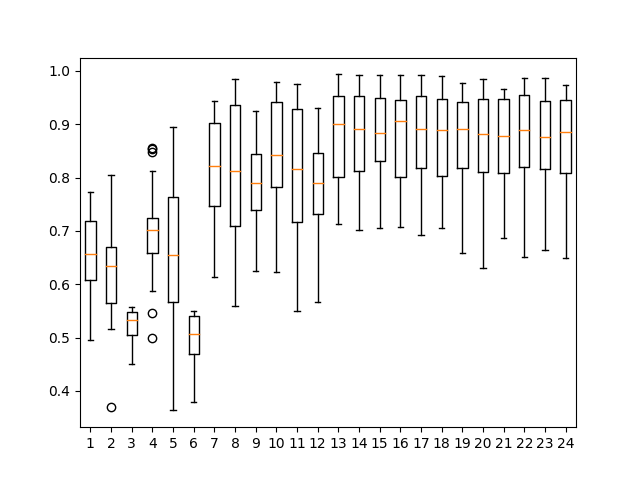
\includegraphics[scale=1]{acc_small_all.png}

\caption{\emph{Accuracy} + reducción de las combinaciones de las metaheurísticas para los conjuntos pequeños}
\label{small-accu-all}
\end{figure}

\newpage

\begin{figure}[h!]

	\centering
	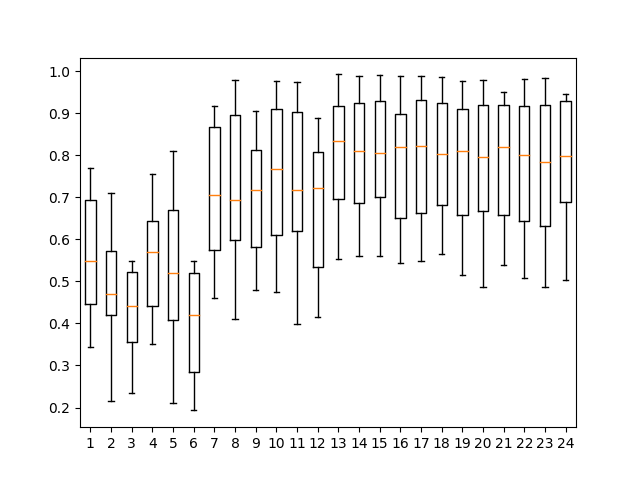
\includegraphics[scale=1]{kappa_small_all.png}

\caption{\emph{Kappa} + reducción de las combinaciones de las metaheurísticas para los conjuntos pequeños}
\label{small-kap-all}
\end{figure}

Los \emph{boxplots} que van desde el número 13 hasta el 18 confirman que todas las combinaciones de MA presentan valores similares. Esto también sucede con CHC al ver los \emph{boxpĺots} que van desde el 19 hasta el 24. Los p-valores de las tablas \ref{wilcox-MA-peq} y \ref{wilcox-CHC-peq} en el anexo A muestran que todas las variantes son estadísticamente similares en \emph{accuracy} + reducción y \emph{kappa} + reducción.

De las figuras \ref{small-accu-all} y \ref{small-kap-all} también se puede apreciar que las combinaciones de MA y las de CHC presentan valores similares. Los resultados de la prueba \emph{Wilcoxon} (ver tabla \ref{wilcox-best-peq} en el anexo A) para MA y CHC muestran p-valores iguales a 6.934e-02 para \emph{accuracy} + reducción y 7.800e-02 para \emph{kappa} + reducción, lo que implica que ambos algoritmos son estadísticamente similares.

Como la diferencia entre MA y CHC es el tiempo de cómputo, se tiene que CHC con población inicial aleatoria presenta los tiempos más cortos y por lo tanto es la mejor metaheurística para resolver el problema de selección de prototipos sobre conjuntos pequeños.


\subsubsection{Conjuntos medianos}

En esta sección se estudia el comportamiento de las combinaciones de GGA, SSGA, MA y CHC al resolver el problema de selección de instancias sobre conjuntos medianos. El objetivo es determinar cuál algoritmo presenta el mayor nivel de \emph{accuracy} + reducción. Además, se estudia el tiempo que requiere cada algoritmo en dar una solución.

\begin{table}[h!]
\centering
\begin{adjustbox}{max width =\textwidth}
\begin{tabular}{l c c c c c c c}
\hline
\multirow{2}{*}{\textsc{Algoritmo}}
	& \multicolumn{2}{c}{\textsc{Accuracy}}
	& \multicolumn{2}{c}{\textsc{Kappa}}
	& \textsc{Reducción}
	& \textsc{Acc + Red}
	& \textsc{Tiempo (seg)} \\
	& Training & Test
	& Training & Test \\ 
\hline
\hline

CNN-GGA     & 79.90 & 70.51 & 59.52 & 44.26 & 77.45 & 147.96 & 232.8342 \\
ENN-GGA     & 84.75 & 80.71 & 69.49 & 59.65 & 28.62 & 109.33 & 125.8465 \\
RSS-GGA     & 80.27 & 75.20 & 55.75 & 45.47 & 67.33 & 142.53 & 137.0381 \\
\textbf{CNN-RSS-GGA} & \textbf{89.32} & \textbf{78.90} & \textbf{75.71} & \textbf{55.16} & \textbf{55.14} & \textbf{134.04} & \textbf{309.4603} \\
ENN-RSS-GGA & 91.41 & 81.55 & 82.46 & 61.68 & 19.81 & 101.36 & 314.2968 \\

\hline

CNN-SSGA & 85.40 & 80.07 & 69.65 & 59.23 & 85.47 & 165.54 & 6.4410 \\
ENN-SSGA & 82.00 & 80.09 & 63.24 & 57.93 & 74.59 & 154.68 & 5.6722 \\
\textbf{RSS-SSGA} & \textbf{83.02} & \textbf{80.45} & \textbf{63.89} & \textbf{58.54} & \textbf{86.90} & \textbf{167.35} & \textbf{5.9946} \\
CNN-RSS-SSGA & 85.86 & 80.47 & 70.43 & 59.77 & 81.21 & 161.68 & 10.5868 \\
ENN-RSS-SSGA & 85.50 & 80.78 & 70.42 & 60.04 & 70.49 & 151.27 & 10.4293 \\

\hline

\textbf{CNN-MA} & \textbf{81.16} & \textbf{80.21} & \textbf{60.00} & \textbf{57.65} & \textbf{95.72} & \textbf{175.93} & \textbf{57.3939} \\
ENN-MA & 79.38 & 79.25 & 57.47 & 56.08 & 97.07 & 176.32 & 67.5310 \\
RSS-MA & 79.24 & 78.93 & 56.11 & 54.49 & 96.71 & 175.64 & 69.5927 \\
CNN-RSS-MA & 80.51 & 80.15 & 59.62 & 58.08 & 96.54 & 176.69 & 121.2220 \\
ENN-RSS-MA & 80.70 & 79.71 & 58.86 & 56.53 & 96.33 & 176.04 & 112.0309 \\

\hline

CNN-CHC & 83.03 & 80.81 & 63.37 & 59.25 & 93.52 & 174.33 & 4.6572 \\
ENN-CHC & 81.07 & 80.32 & 60.84 & 58.34 & 93.56 & 173.88 & 5.0976 \\
\textbf{RSS-CHC} & \textbf{81.51} & \textbf{80.58} & \textbf{60.74} & \textbf{58.51} & \textbf{95.35} & \textbf{175.93} & \textbf{4.7450} \\
CNN-RSS-CHC & 82.76 & 80.73 & 62.80 & 58.71 & 93.19 & 173.92 & 6.7859 \\
ENN-RSS-CHC  & 82.55 & 80.74 & 63.55 & 59.44 & 91.54 & 172.28 & 7.0284 \\


\hline
\end{tabular}
\end{adjustbox}
\caption{Promedios de los resultados obtenidos en las distintas métricas para las distintas combinaciones de cada metaheurística sobre los conjuntos pequeños}
\label{med-all}

\end{table}

Al estudiar los resultados obtenidos en la tabla \ref{med-all}, se pueden destacar los siguientes aspectos observados de las combinaciones de GGA:

\begin{itemize}

\item CNN-GGA y RSS-GGA no son tomados en cuenta por tener un \emph{kappa} por debajo de 50\%.

\item CNN-RSS-GGA presenta el mayor nivel de \emph{acuracy} + reducción.

\item ENN-GGA y RSS-GGA son las combinaciones que menos tiempo toman en dar un resultado.

\end{itemize}

De las observaciones anteriores se puede concluir que CNN-RSS-GGA es la mejor combinación de GGA ya que presenta el mayor valor de \emph{accuracy} + reducción, mientras presenta un \emph{kappa} superior al 50\%.

Al estudiar las combinaciones de SSGA, se tiene que RSS-SSGA y CNN-SSGA presentan los mayores valores en \emph{accuracy} + reducción. Como los resultados entre las dos metaheurísticas son muy similares, se necesita evaluar los p-valores de la prueba \emph{Wilcoxon}. En la tabla \ref{wilcox-SSGA-med} del apéndice A se puede apreciar que el p-valor de la comparación entre RSS-SSGA y CNN-SSGA en \emph{accuracy} + reducción es de 2.772e-01, lo que implica que ambas metaheurísticas son estadísticamente similares. Por lo tanto, ya que RSS-SSGA toma menos tiempo en dar un resultado, puede ser considerarada como la mejor combinación de SSGA.

Al estudiar las combinaciones de MA, se observa que todas presentan \emph{accuracy + reducción} similares y los p-valores de las tablas \ref{wilcox-MA-med} en el apéndice A corroboran este hecho. Por lo tanto, se elige CNN-MA como la mejor combinación de MA por ser la que presenta el tiempo de cómputo más corto.

Al analizar los resultados de las combinaciones de CHC, se tiene que RSS-CHC, CNN-CHC y ENN-CHC presentan los mayores valores de \emph{accuracy} + reducción. Los p-valores de la tabla \ref{wilcox-CHC-med} muestran que estas tres combinaciones son estadísticamente similares en \emph{accuracy} + reducción. Por lo tanto, se puede considerar RSS-CHC como la mejor de CHC, ya que es de las que tarda menos tiempo.

En la tabla \ref{med-best-all} se comparan las mejores combinaciones de cada metaheurística con su versión original (población inicial aleatoria). La idea es determinar si la mejor combinación representa una mejoría sobre la versión original. De esta tabla se puede llegar a las siguientes conclusiones:

\begin{table}[h!]
\centering
\begin{adjustbox}{max width =\textwidth}
\begin{tabular}{l c c c c c c c}
\hline
\multirow{2}{*}{\textsc{Algoritmo}}
	& \multicolumn{2}{c}{\textsc{Accuracy}}
	& \multicolumn{2}{c}{\textsc{Kappa}}
	& \textsc{Reducción}
	& \textsc{Acc + Red}
	& \textsc{Tiempo (seg)} \\
	& Training & Test
	& Training & Test \\ 
\hline
\hline

\textbf{GGA}  & \textbf{87.02} & \textbf{79.82} & \textbf{73.75} & \textbf{58.12} & \textbf{56.41} & \textbf{136.23} & \textbf{110.0812} \\
CNN-RSS-GGA & 89.32 & 78.90 & 75.71 & 55.16 & 55.14 & 134.04 & 309.4603 \\

\hline

SSGA & 84.31 & 80.29 & 66.76 & 58.71 & 83.92 & 164.21 & 3.5589 \\
\textbf{RSS-SSGA} & \textbf{83.02} & \textbf{80.45} & \textbf{63.89} & \textbf{58.54} & \textbf{86.90} & \textbf{167.35} & \textbf{5.9946} \\

\hline

MA   & 80.57 & 79.08 & 58.25 & 55.64 & 96.24 & 175.32 & 73.3461 \\
\textbf{CNN-MA} & \textbf{81.16} & \textbf{80.21} & \textbf{60.00} & \textbf{57.65} & \textbf{95.72} & \textbf{175.93} & \textbf{57.3939} \\

\hline

\textbf{CHC}  & \textbf{83.13} & \textbf{81.15} & \textbf{63.47} & \textbf{59.86} & \textbf{94.55} & \textbf{175.7}  & \textbf{2.8843} \\
RSS-CHC & 81.51 & 80.58 & 60.74 & 58.51 & 95.35 & 175.93 & 4.7450 \\

\hline
\end{tabular}
\end{adjustbox}
\caption{Comparación entre los resultados de las métricas obtenidas por la metahuerística original y la mejor combinación para los conjuntos medianos}
\label{med-best-all}

\end{table}

\begin{itemize}
 
\item Al comparar CNN-RSS-GGA con GGA en \emph{accuracy} + reducción se tiene que el p-valor de la tabla \ref{wilcox-gga-med} en el apéndice A es 1. Lo que significa que estadísticamente ambas metaheurísticas son iguales. La diferencia está en el tiempo de cómputo, donde CNN-RSS-GGA tarda aproximadamente 3 veces el tiempo de GGA. Por lo tanto, se concluye que CNN-RSS-GGA no representa una mejoría sobre GGA.

\item RSS-SSGA presenta un mayor valor de \emph{accuracy} + reducción que SSGA, principalmente por tener una tasa de reducción 2.98\% por encima de SSGA, mientras mantiene niveles similares de \emph{accuracy y kappa}. Al hacer la prueba de \emph{Wilcoxon} para \emph{accuracy} + reducción se obtiene el p-valor 7.013e-03 (ver tabla \ref{wilcox-SSGA-med} en el apéndice A), lo que significa que hay una diferencia real entre RSS-SSGA y SSGA. Estas razones justifican el tiempo adicional de cómputo de RSS-GGA, por lo que se determina como una mejoría real sobre SSGA.

\item Los valores de \emph{accuracy} + reducción son similares entre MA y CNN-MA. El p-valor de la prueba estadística es 1 (ver tabla \ref{wilcox-MA-med} en el apéndice A), por lo que son estadísticamente iguales. La diferencia se encuentra en el tiempo de cómputo, en cuyo caso CNN-MA tarda menos en devolver un resultado, esto se debe a que con la población proporcionada por CNN se disminuyó el número de veces que MA utilizó el proceso de optimización interna. En conclusión, CNN-MA representa una mejoría sobre MA, ya que disminuye los tiempos de cómputo manteniendo el mismo valor de \emph{accuracy} + reducción.

\item  Los valores de \emph{accuracy} + reducción son similares entre CHC y RSS-CHC. El p-valor de la prueba estadística es 9.679e-01 (ver tabla \ref{wilcox-CHC-med} en el apéndice A), por lo que no hay una diferencia significativa. Por lo tanto, RSS-CHC no representa una mejora sobre CHC, ya que sólo aumenta el tiempo de cómputo.

\end{itemize}

\begin{table}[h!]
\centering
\begin{adjustbox}{max width =\textwidth}
\begin{tabular}{l c c|l c c}
\hline
\multicolumn{3}{c|}{\textsc{Accuracy + Reducción}}
	& \multicolumn{3}{c}{\textsc{Kappa + Reducción}}\\
\hline
Algoritmo & Rango & Mejor & Algoritmo & Rango & Mejor \\
\hline
\hline

CNN-RSS-MA   & 4.76  & 5 & CHC          & 5.05  & 2 \\
ENN-MA       & 5.05  & 4 & ENN-MA       & 5.41  & 4\\
CHC          & 5.52  & 2 & CNN-RSS-MA   & 5.52  & 5\\
CNN-MA       & 5.94  & 3 & RSS-CHC      & 6.52  & 0\\
ENN-RSS-MA   & 5.94  & 1 & CNN-MA       & 6.76  & 2\\
RSS-CHC      & 5.94  & 0 & ENN-RSS-MA   & 7.05  & 1\\
MA           & 6.29  & 0 & MA           & 7.23  & 1\\
RSS-MA       & 7.05  & 1 & CNN-CHC      & 7.23  & 0\\
CNN-CHC      & 7.35  & 0 & ENN-CHC      & 7.47  & 1\\
ENN-CHC      & 8.41  & 0 & CNN-RSS-CHC  & 8.29  & 0\\
CNN-RSS-CHC  & 8.70  & 0 & RSS-MA       & 8.41  & 0 \\
ENN-RSS-CHC  & 10.00 & 1 & ENN-RSS-CHC  & 8.47  & 1 \\
RSS-SSGA     & 13.47 & 0 & CNN-SSGA     & 12.94 & 0 \\
CNN-SSGA     & 13.47 & 0 & RSS-SSGA     & 13.05 & 0 \\
SSGA         & 14.70 & 0 & SSGA         & 14.23 & 0 \\
CNN-RSS-SSGA & 15.82 & 0 & CNN-RSS-SSGA & 15.05 & 0 \\
ENN-SSGA     & 16.64 & 0 & ENN-SSGA     & 16.76 & 0 \\
CNN-GGA      & 18.17 & 0 & ENN-RSS-SSGA & 18.00 & 0 \\
ENN-RSS-SSGA & 18.47 & 0 & CNN-GGA      & 18.52 & 0 \\
RSS-GGA      & 19.94 & 0 & GGA          & 20.47 & 0 \\
GGA          & 21.00 & 0 & RSS-GGA      & 20.52 & 0 \\
CNN-RSS-GGA  & 21.41 & 0 & CNN-RSS-GGA  & 21.23 & 0 \\
ENN-GGA      & 22.05 & 0 & ENN-GGA      & 22.05 & 0 \\
ENN-RSS-GGA  & 23.82 & 0 & ENN-RSS-GGA  & 23.64 & 0  \\

\hline
\end{tabular}
\end{adjustbox}
\caption{Rangos de las metaheurísticas en \emph{accuracy + reducción}, \emph{kappa + reducción} y tiempo para los conjuntos medianos}
\label{rank-med}
\end{table}

La tabla \ref{rank-med} muestra que las combinaciones de MA y CHC obtienen los mayores niveles de \emph{accuracy} + reducción y \emph{kappa} + reducción. CHC con población inicial aleatoria destaca por ocupar los primeros puestos, sin embargo las combinaciones de MA contabilizan la mayor cantidad de conjuntos para los cuales han obtenido los mejores valores.

\newpage

Las figuras \ref{medium-accu-all} y \ref{medium-kap-all} muestran \emph{boxplots} de todas las combinaciones de metaheurísticas para los conjuntos medianos, de izquierda a derecha los \emph{boxplots} representan las siguientes combinaciones: '1':GGA, '2':CNN-GGA, '3':ENN-GGA, '4':RSS-GGA, '5':CNN-RSS-GGA, '6':ENN-RSS-GGA, '7':SSGA, '8':CNN-SSGA, '9':ENN-SSGA, '10':RSS-SSGA, '11':CNN-RSS-SSGA, '12':ENN-RSS-SSGA, '13':MA, '14':CNN-MA, '15':ENN-MA, '16':RSS-MA, '17':CNN-RSS-MA, '18':ENN-RSS-MA, '19':CHC, '20':CNN-CHC, '21':ENN-CHC, '22':RSS-CHC, '23':CNN-RSS-CHC y '24':ENN-RSS-CHC.

\begin{figure}[h!]

	\centering
	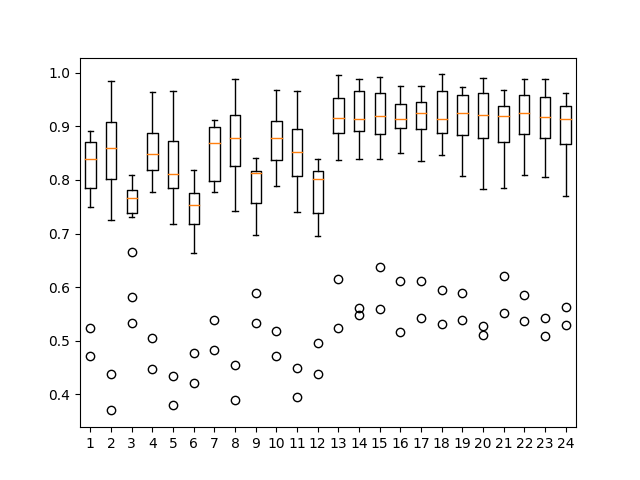
\includegraphics[scale=0.8]{acc_medium_all.png}

\caption{\emph{Accuracy} + reducción de las combinaciones de las metaheurísticas para los conjuntos medianos}
\label{medium-accu-all}
\end{figure}


\begin{figure}[h!]

	\centering
	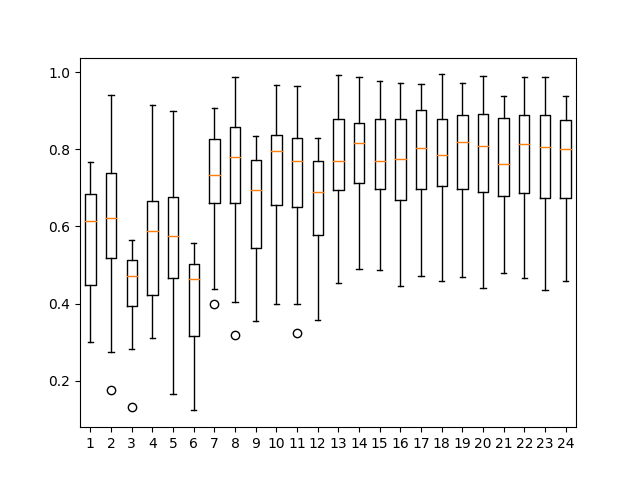
\includegraphics[scale=0.8]{kappa_medium_all.png}

\caption{\emph{Kappa} + reducción de las combinaciones de las metaheurísticas para los conjuntos medianos}
\label{medium-kap-all}
\end{figure}

Los \emph{boxplots} que van desde el número 13 hasta el 18 confirman que todas las combinaciones de MA presentan valores similares. Los p-valores de la tabla \ref{wilcox-MA-med} en el anexo A muestran que todas las combinaciones de MA son estadísticamente similares en \emph{accuracy} + reducción y \emph{kappa} + reducción.

Los \emph{boxpĺots} que van desde el 19 hasta el 24 muestran similitud entre las combinaciones de CHC. Al evaluar los p-valores de la tabla \ref{wilcox-CHC-med} del anexo A se tiene que CHC, CNN-CHC, ENN-CHC y RSS-CHC son estadísticamente similares, mientras que CNN-RSS-CHC y ENN-RSS-CHC son distintos al resto; esto es porque presentan niveles más bajo de reducción.

De las figuras \ref{medium-accu-all} y \ref{medium-kap-all} también se puede apreciar que las combinaciones de MA y las de CHC presentan valores similares. Los resultados de la prueba \emph{Wilcoxon} (ver tabla \ref{wilcox-best-med} en el anexo A) para CNN-MA y CHC muestran p-valores iguales a 6.292e-01 para \emph{accuracy} + reducción y 5.197e-01 para \emph{kappa} + reducción, lo que implica que ambos algoritmos son estadísticamente similares.

Como la diferencia entre CNN-MA y CHC es el tiempo de cómputo, se tiene que CHC con población inicial aleatoria presenta los tiempos más cortos y por lo tanto es la mejor metaheurística para resolver el problema de selección de prototipos sobre conjuntos medianos.


\subsubsection{Conjuntos Grandes}

En esta sección se estudia el comportamiento de las combinaciones de GGA, SSGA, MA y CHC al resolver el problema de selección de instancias sobre conjuntos grandes. El objetivo es determinar cuál algoritmo presenta los mayores niveles de \emph{accuracy} + reducción. Además, se estudia el tiempo que requiere cada algoritmo en dar una solución.

\begin{table}[h!]
\centering
\begin{adjustbox}{max width =\textwidth}
\begin{tabular}{l c c c c c c c}
\hline
\multirow{2}{*}{\textsc{Algoritmo}}
	& \multicolumn{2}{c}{\textsc{Accuracy}}
	& \multicolumn{2}{c}{\textsc{Kappa}}
	& \textsc{Reducción}
	& \textsc{Acc + Red}
	& \textsc{Tiempo (seg)} \\
	& Training & Test
	& Training & Test \\ 
\hline
\hline

CNN-GGA     & 71.06 & 64.31 & 44.78 & 30.94 & 84.09 & 148.4 & 1568.8913 \\
ENN-GGA     & 93.57 & 88.90 & 79.44 & 64.53 & 15.02 & 103.92 & 718.0400 \\
\textbf{RSS-GGA}     & \textbf{91.50} & \textbf{87.19} & \textbf{72.27} & \textbf{58.21} & \textbf{70.83} & \textbf{158.02} & \textbf{1197.0505} \\
CNN-RSS-GGA & 94.55 & 85.88 & 84.10 & 58.85 & 60.89 & 146.77 & 2646.6438 \\
ENN-RSS-GGA & 95.74 & 87.98 & 86.69 & 62.38 & 10.25 & 98.23 & 1703.4263 \\

\hline

CNN-SSGA & 88.97 & 85.12 & 70.02 & 59.39 & 88.07 & 173.19 & 90.1004 \\
ENN-SSGA & 90.97 & 88.92 & 71.13 & 64.41 & 68.23 & 157.15 & 34.9024 \\
\textbf{RSS-SSGA} & \textbf{89.68} & \textbf{88.26} & \textbf{67.43} & \textbf{62.71} & \textbf{89.27} & \textbf{177.53} & \textbf{57.7995} \\
CNN-RSS-SSGA & 90.02 & 86.34 & 71.40 & 60.69 & 84.34 & 170.68 & 99.1629 \\
ENN-RSS-SSGA & 91.12 & 88.05 & 72.45 & 62.72 & 66.68 & 154.73 & 78.5967 \\

\hline

CNN-MA & 89.25 & 89.26 & 63.60 & 63.41 & 98.84 & 188.1 & 612.7902 \\
ENN-MA & 88.07 & 89.02 & 60.72 & 61.45 & 99.76 & 188.78 & 288.6525 \\
RSS-MA & 90.00 & 90.02 & 63.47 & 63.43 & 97.46 & 187.48 & 527.9115 \\
CNN-RSS-MA & 88.57 & 89.51 & 61.76 & 61.60 & 97.07 & 186.58 & 960.3951 \\
ENN-RSS-MA & 87.46 & 89.12 & 62.92 & 63.86 & 99.69 & 188.81 & 443.0003 \\

\hline

CNN-CHC & 89.03 & 88.71 & 65.54 & 64.37 & 97.71 & 186.42 & 38.3314 \\
ENN-CHC & 89.93 & 89.64 & 67.46 & 66.31 & 92.33 & 181.97 & 27.3520 \\
RSS-CHC & 89.72 & 89.62 & 65.91 & 65.26 & 98.19 & 187.81 & 41.1142 \\
CNN-RSS-CHC & 89.45 & 89.10 & 89.45 & 64.35 & 97.19 & 186.29 & 50.5800 \\
ENN-RSS-CHC & 89.75 & 89.22 & 67.21 & 65.32 & 90.99 & 180.21 & 47.4006 \\

\hline
\end{tabular}
\end{adjustbox}
\caption{Promedios de los resultados obtenidos en las distintas métricas para las distintas combinaciones de cada metaheurística sobre los conjuntos pequeños}
\label{grande-all}

\end{table}

Al estudiar los resultados obtenidos en la tabla \ref{grande-all}, se puede destacar, referente a GGA, que RSS-GGA presenta el mayor nivel de \emph{accuracy} + reducción. Además, RSS-GGA se encuentra entre las combinaciones que toman menos tiempo en regresar un resultado. Por lo tanto, se puede considerar a RSS-GGA como la mejor combinación de GGA.

Al analizar a los resultados obtenidos para las combinaciones de SSGA, se puede observar que RSS-SSGA presenta el mayor valor de \emph{accuracy} + reducción. Además, junto con ENN-SSGA, presentan los tiempos más cortos de cómputo. 

Al evaluar los resultados obtenidos por las combinaciones de MA, se observa que todas presentan \emph{accuracy} + reducción similares. Por lo tanto, la elección de cuál es la mejor combinación para cada metaheurística se debe hacer en función al tiempo de cómputo, donde ENN-MA sobresale por ser la que presenta el menor tiempo.

Al estudiar los resultados obtenidos por las combinaciones de CHC, se observa que CNN-CHC, RSS-CHC y CNN-RSS-CHC obtienen los mayores niveles de \emph{accuracy} + reducción. En consecuencia, se elige CNN-CHC como la mejor combinación ya que presenta los tiempos de cómputo más cortos.


En la tabla \ref{large-best-all} se comparan las mejores combinaciones de cada metaheurística con su versión original (población inicial aleatoria). La idea es determinar si la mejor combinación representa una mejoría sobre la versión original. De esta tabla se puede llegar a las siguientes conclusiones:

\begin{table}[h!]
\centering
\begin{adjustbox}{max width =\textwidth}
\begin{tabular}{l c c c c c c c}
\hline
\multirow{2}{*}{\textsc{Algoritmo}}
	& \multicolumn{2}{c}{\textsc{Accuracy}}
	& \multicolumn{2}{c}{\textsc{Kappa}}
	& \textsc{Reducción}
	& \textsc{Acc + Red}
	& \textsc{Tiempo (seg)} \\
	& Training & Test
	& Training & Test \\ 
\hline
\hline

GGA  & 93.16 & 86.44 & 79.94 & 60.14 & 50.50 & 136.94 & 672.0273 \\
\textbf{RSS-GGA}     & \textbf{91.50} & \textbf{87.19} & \textbf{72.27} & \textbf{58.21} & \textbf{70.83} & \textbf{158.02} & \textbf{1197.0505} \\

\hline

SSGA & 89.11 & 87.43 & 69.53 & 62.01 & 80.56 & 167.99 & 27.6637 \\
\textbf{RSS-SSGA} & \textbf{89.68} & \textbf{88.26} & \textbf{67.43} & \textbf{62.71} & \textbf{89.27} & \textbf{177.53} & \textbf{57.7995} \\

\hline

\textbf{MA}   & \textbf{89.04} & \textbf{89.99} & \textbf{64.99} & \textbf{65.10} & \textbf{99.73} & \textbf{189.72} & \textbf{256.1432} \\
ENN-MA & 88.07 & 89.02 & 60.72 & 61.45 & 99.76 & 188.78 & 288.6525 \\

\hline

\textbf{CHC}  & \textbf{89.61} & \textbf{89.34} & \textbf{66.14} & \textbf{65.06} & \textbf{96.15} & \textbf{185.76} & \textbf{16.8665} \\
CNN-CHC & 89.03 & 88.71 & 65.54 & 64.37 & 97.71 & 186.42 & 38.3314 \\

\hline
\end{tabular}
\end{adjustbox}
\caption{Comparación entre los resultados de las métricas obtenidas por la metahuerística original y la mejor combinación para los conjuntos grandes}
\label{large-best-all}

\end{table}

\begin{itemize}

\item RSS-GGA presenta un mayor valor de \emph{accuracy} + reducción que GGA, producto de un aumento de la tasa de reducción, la cual es 20.33\% mayor, a la vez que mantiene los mismos niveles de \emph{accuracy y kappa}. Por lo tanto, RSS-GGA representa una mejoría sobre GGA.

\item RSS-SSGA presenta un mayor valor de \emph{accuracy} + reducción que SSGA, producto de un aumento de la tasa de reducción, la cual es 8.71\% mayor, a la vez que mantiene los mismos niveles de \emph{accuracy y kappa}. Por lo tanto, RSS-SSGA representa una mejoría sobre SSGA.

\item Los valores obtenidos por MA y ENN-MA en \emph{accuracy} + reducción son similares. Por lo tanto, ENN-MA no representa una mejora sobre MA y sólo aumenta el tiempo de cómputo.

\item  Los valores obtenidos por CHC y CNN-CHC en \emph{accuracy} + reducción son similares. Por lo tanto, CNN-CHC no representa una mejora sobre CHC y sólo aumenta el tiempo de cómputo.

\end{itemize}

\newpage

\begin{table}[]
\centering
\begin{adjustbox}{max width =\textwidth}
\begin{tabular}{l c c|l c c}
\hline
\multicolumn{3}{c|}{\textsc{Accuracy + Reducción}}
	& \multicolumn{3}{c}{\textsc{Kappa + Reducción}} \\
\hline
Algoritmo & Rango & Mejor & Algoritmo & Rango & Mejor \\
\hline
\hline

MA           & 1.50  & 1 & CNN-MA       & 2.00  & 1 \\
ENN-MA       & 3.00  & 0 & MA           & 2.00  & 0 \\
ENN-RSS-MA   & 3.50  & 1 & ENN-RSS-MA   & 3.00  & 1 \\
CNN-MA       & 5.00  & 0 & RSS-CHC      & 4.50  & 0 \\
RSS-MA       & 5.50  & 0 & CNN-CHC      & 6.50  & 0 \\
RSS-CHC      & 7.00  & 0 & ENN-MA       & 8.00  & 0 \\
CNN-RSS-MA   & 7.50  & 0 & RSS-MA       & 8.00  & 0 \\
CNN-CHC      & 7.50  & 0 & CHC          & 8.00  & 0 \\
CHC          & 9.00  & 0 & CNN-RSS-CHC  & 8.50  & 0 \\
CNN-RSS-CHC  & 9.00  & 0 & ENN-CHC      & 9.50  & 0 \\
CNN-SSGA     & 11.00 & 0 & CNN-SSGA     & 10.50 & 0 \\
ENN-CHC      & 11.50 & 0 & CNN-RSS-MA   & 11.50 & 0 \\
RSS-SSGA     & 12.50 & 0 & ENN-RSS-CHC  & 12.50 & 0 \\
ENN-RSS-CHC  & 13.50 & 0 & RSS-SSGA     & 12.50 & 0 \\
CNN-RSS-SSGA & 15.00 & 0 & CNN-RSS-SSGA & 15.00 & 0 \\
SSGA         & 15.50 & 0 & SSGA         & 15.50 & 0 \\
RSS-GGA      & 17.50 & 0 & ENN-SSGA     & 17.50 & 0 \\
ENN-SSGA     & 18.00 & 0 & RSS-GGA      & 18.00 & 0 \\
ENN-RSS-SSGA & 19.00 & 0 & ENN-RSS-SSGA & 18.50 & 0 \\
CNN-GGA      & 19.50 & 0 & CNN-RSS-GGA  & 20.00 & 0 \\
CNN-RSS-GGA  & 20.00 & 0 & CNN-GGA      & 20.50 & 0 \\
GGA          & 21.50 & 0 & GGA          & 21.00 & 0 \\
ENN-GGA      & 23.50 & 0 & ENN-GGA      & 23.50 & 0 \\
ENN-RSS-GGA  & 23.50 & 0 & ENN-RSS-GGA  & 23.50 & 0 \\

\hline
\end{tabular}
\end{adjustbox}
\caption{Rangos de las metaheurísticas en \emph{accuracy + reducción}, \emph{kappa + reducción} y tiempo para los conjuntos grandes}
\label{rank-large}
\end{table}

La tabla \ref{rank-large} muestra que las combinaciones de MA y CHC obtienen los mayores niveles de \emph{accuracy} + reducción y \emph{kappa} + reducción. Donde las combinaciones de MA contabilizan la mayor cantidad de conjuntos para los cuales han obtenido los mejores valores. La tabla \ref{meta}, muestra que la diferencia entre MA y CHC está en la tasa de reducción, donde MA supera en 3.58\% a CHC. Sin embargo, si se toma en cuenta que MA tarda 15 veces más para resolver el problema y que CHC es la metaheurística más rápida; se puede concluir que CHC es la mejor metaheurística para resolver el problema de selección de prototipos sobre conjuntos grandes.
